%%%%%%%%%%%%%%%%%%%%%%%%%%%%%%%%%%%%%%%%%%%%%%%%%%%%%%%%%%%%%%%%%
%%%  Capstone Project Template that tries to save a few trees %%%
%%%  Edwin Blake 22 Aug 2013                                  %%%
%%%		1 Aug 2014 (revised)                                  %%%
%%%             10 Aug 2015                                   %%%
%%%  see also                                                 %%%
%%% http://ravirao.wordpress.com/2005/11/19/latex-tips-to-meet-publication-page-limits/
%%%%%%%%%%%%%%%%%%%%%%%%%%%%%%%%%%%%%%%%%%%%%%%%%%%%%%%%%%%%%%%%%

\documentclass[11pt,a4paper]{article}
\usepackage{times}
% Allows better control over headers and footers
\usepackage{fancyhdr}
% set the margins using the geometry package (which is much the easiest way of
% doing this).
\usepackage[margin=2.5cm]{geometry}
% Pictures (means you have to produce pdf output via pdflatex)
\usepackage[pdftex]{graphicx}
% Set a default path for the image files
\graphicspath{{./images/}}
% Clickable hyperlinks
\usepackage{hyperref}
% Try to reduce the white space latex loves so much
\usepackage[small,compact]{titlesec}
% Reduce space around section heads and add a full stop after the number
\titlelabel{\thetitle. \quad}
% Use fancy headers
\pagestyle{fancy}
% Change name of Abstract to nothing and loose some of the excessive white
% space
\renewcommand{\abstractname}{\vskip -5mm}

\begin{document}
\title{Final Report: RoboViz Capstone Project} \date{}
\author{Boyd Kane\\KNXBOY001\\KNXBOY001@myuct.ac.za
\and Imaad Ghoor\\GHRIMA002\\GHRIMA002@myuct.ac.za
\and Jesse Sarembock\\SRMJES001\\SRMJES001@myuct.ac.za}

%  Set the headers via fancyhdr package
% Short title for running head
\lhead{RoboViz Final Report}
\chead{}
\lfoot{}
% add page number as centre footer.
\cfoot{\thepage}
\rfoot{}
% Don't want horizontal line under header
\renewcommand{\headrulewidth}{0.0pt}

\maketitle
% First page is plain style headings and footers (ie just the page number as
% footer).
\thispagestyle{plain}

\begin{abstract}
% First you should have an executive summary (or abstract) just a single
% paragraph saying what the results of the project are (at most 200
% words).
    This Final Report describes the 2021 RoboViz Capstone project completed by
    third year computer science students. This project expanded on the open
    source RoboGen software to add the ability to simulate multiple robots in a
    swarm, among other extensions.
\end{abstract}

% We expect a report of about 3500-4000 words, written single spaced, with a font
% size of at least 11 pts.  Use at least a 2.5 cm margin on all sides of the
% pages.
%
% No blank lines between paragraphs except to get figures and their captions to
% position properly.
%
% Depending on how many diagrams you use (more is better) the report will be
% between 7 and 10 pages long. Your appendices (e.g., user manual, test results,
% which are needed) are not included in these limits.
%
% You must had-in an Adobe Acrobat file for your report (i.e., pdf
% file).
% You should begin your write-up with an overview and then drill down
% into the details of what you produced. Your report should cover the
% following sections (Sections \ref{s:introduction} --
% \ref{s:conclusion}).
%
% Some notes about code formatting
% - Each method should start with a brief description of its
%   function.
% - Use indentation to display the structure within a method.
% - Comments should be used extensively. They are best used to
%   describe logical blocks of code rather than individual
%   statements. Line-by-line comments have the drawbacks of not
%   providing any overview and of decreasing readability.
% - Meaningful identifiers should be chosen.
% - Output should be pleasingly formatted and easy to read.
%
% You do, of course, have the option to call in any of your
% favourite packages for setting maths, graphics, computer listings,
% etc.

\tableofcontents
\section{Introduction}
\label{s:introduction}
% Your introduction provides the context for the project and should
% contain the statement of the scope of the project (which may have
% changed since you first wrote it). Someone reading your introduction
% must have clear idea of what the system is intended for. If you think
% there is something special about the kind of problem you tackled that
% your reader needs to know up front then this is where you say it.
%
% If you need any survey of other work (you probably don't) then put it
% towards the end of the introduction and give suitable references. A
% case where this is needed is if your project builds on someone else's
% project or some published algorithm.
%
% Discuss your approach to solving the problem. Please give a short
% overview of the software engineering methods you used (e.g.,
% traditional analysis followed by design and implementation -- typically
% the case if you did an evolutionary prototype, or a more agile
% approach where you had a cyclical development process).

This project - RoboViz - involves extending an existing visualiser (RoboGen) to
enable the visualisation of multiple of multiple robots simultaneously.
Robogen allows researchers to define a robot structure and then make use of
genetic algorithms (paired with a fitness function) to evolve robots that that
gradually perform better (as a measured by the relevant fitness function) as
more generations of robots are simulated.


After a set number of generations, the final robot can also be visualised,
although currently the software only allows for the visualisation of a single
robot. The software also generates STL files which describe the 3D body parts
of the robot, such that a 3D printer can take those files and 3D print the body
components of the evolved robot. INO files are also generated, which can be
loaded onto the Arduino platform and define the robot’s ‘brain’ as a software
defined artificial neural network which was evolved by the genetic algorithm.


This project involves modifying the source code of the RoboGen software and
proving that the modifications are efficient enough for at least 3 (but
preferably more) robots to be simulated at once.


An agile software development approach was taken to develop this project. The
project team has worked over WhatsApp and MS Teams, informing each other on
their work and designating tasks from there. Time was spent on creating
functional code to implement a swarm of robots and testing that code before
adding more functionality. The team has had frequent meetings with project
stakeholders, receiving feedback directly from the stakeholders while
developing the project. Throughout development, there have been a significant
number of changes needed as development progressed and these were added to the
project plan over time.


A vertical prototype was chosen for this project since it focuses on
implementing a specific feature - swarm of robots in the visualiser - this was
the most appropriate prototype as it tests key components during early stages
of the project to check key functions.

\section{Requirements Captured}
% The next section deals with the analysis of your system. Cover the
% functional, non-functional and usability requirements. This is where
% you present your use case narratives and diagrams.

% Discuss the major analysis artefacts that you produced. We will expect
% you to produce at least one overall description of the architecture
% used in your system as a diagram, either here or below (see Section
% \ref{s:design-overview}). You may also want to include an analysis
% class hierarchy diagram.

This section provides an overview of the system and discusses functional,
non-functional and usability requirements.

\subsection{Functional Requirements}


\begin{itemize}
  \item Defines robots in a visualiser
  \item Defines robot behaviour in a visualiser
  \item Visualizes a swarm of robots performing a task
  \item
\end{itemize}

\subsection{Non-functional Requirements}


\begin{itemize}
  \item Takes in parameters for a robot file and a test scenario and starts
      simulating that robot
  \item
\end{itemize}


\subsection{Usability Requirements}

\subsection{Use Case Diagram}

\begin{figure}[htpb]
\centering
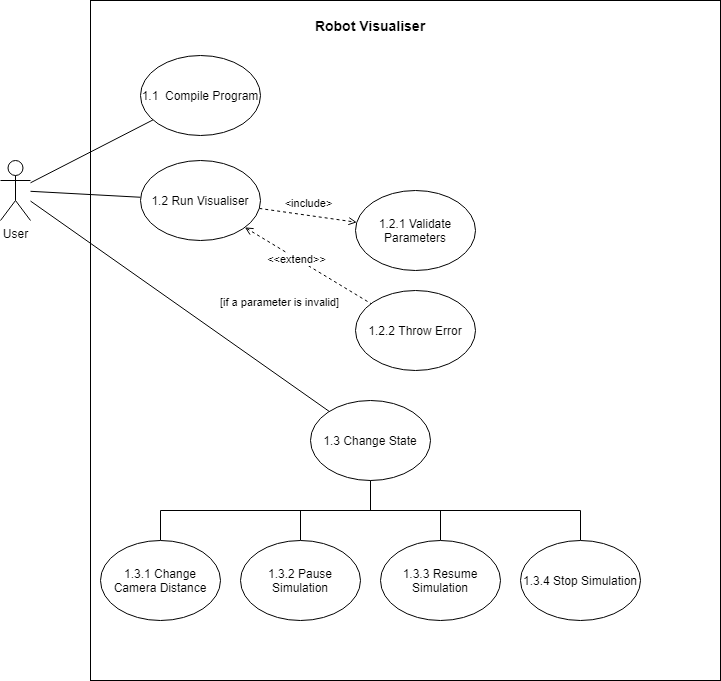
\includegraphics[width=0.8\textwidth]{2}
\caption{Use Case Diagram}
\label{fig:use-case-diagram}
\end{figure}

see figure
\ref{fig:use-case-diagram}

\subsection{Use Case Narratives}
\subsubsection{Start Simulation of the Swarm. Actor: User}
\paragraph{Primary Path:} The user runs the program and is prompted to enter
the name of a robot file and a configuration file (which includes how many
robots to simulate in the swarm).  The program loads a new window that is the
visualiser, and displays the specified number of robots performing their tasks
from the same robot file.  While the simulation is running, the user may pause
the simulation and zoom into the area where the robots are performing for a
closer view.

\paragraph{Alternative Path:} If the robot file entered is incorrectly
formatted or does not exist then the program will throw an error and return the
command line help page.

\subsubsection{ Run Visualiser. Actor: User}
\paragraph{Primary Path:} The user starts the visualiser, after that, the user
needs to enter 2 parameters, location of the file that defines the robot and
the location of the file that defines requirements and configurations for the
file viewer. Should one of the parameters entered be invalid or non-existent,
an exception will be thrown, requiring the user to enter those parameters
again.

\subsubsection{ View Simulation. Actor: User}
\paragraph{Primary Path:} Once the simulation displays the robots performing
their tasks in the run-time environment. The user may change the state of the
view, by pausing,resuming and stopping the simulation. The user may also zoom
in closer to the robots or zoom further away. The simulation will stop once the
time limit specified in the configuration file has passed.

\section{Design Overview}
\label{s:design-overview}
% The next section is an overview of your design. The system design has
% to be justified in terms of the expected behaviour of the final
% product.
%
% If you produced a design class diagram put it here.
% \begin{figure}[h!]
%   \center{\includegraphics[scale=0.8]{architecture.png}}
%   \caption{An architecture diagram. Caption to go below figure}
%   \label{fig:architecture}
% \end{figure}
%
% You must present the overall architecture of the system together with
% an architecture diagram. You may choose what kind of diagram best
% suits your project but we would expect a layered architecture diagram
% (see Figure \ref{fig:architecture}) unless there is a good reason for
% some other kind of diagram. It need not be a formal UML diagram as
% long as it conveys all the necessary information clearly.
%
% You should then (in subsections) cover the algorithms and the data
% organisation used and why they were considered the best.

This section provides a few diagrams that showcase the overall system design.
Figure \ref{fig:analysis-class-diagram} shows the Analysis Class Diagram of the
project.

\begin{figure}[htpb]
    \centering
    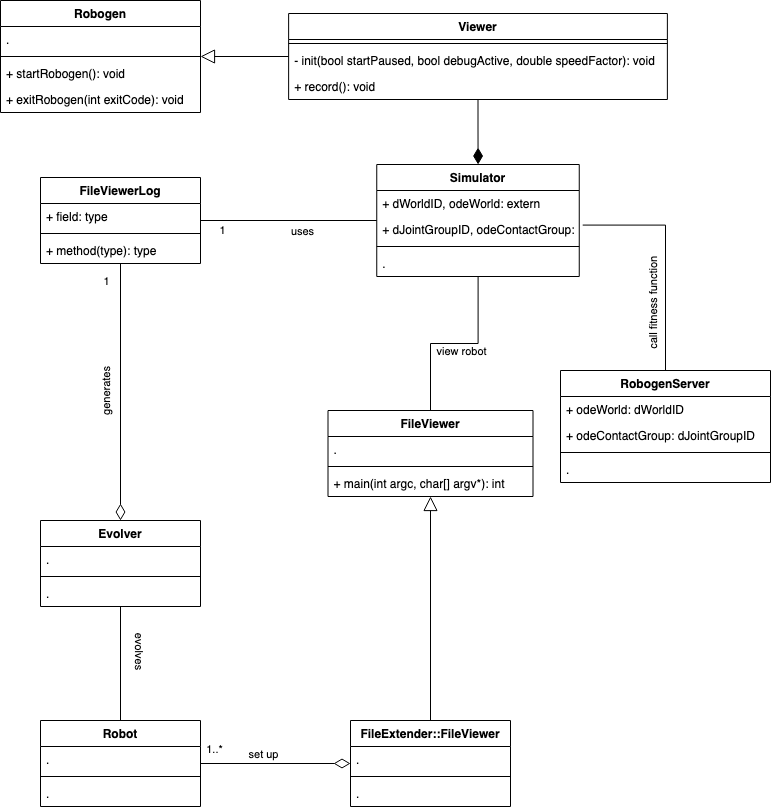
\includegraphics[width=0.8\textwidth]{1}
    \caption{Analysis Class diagram}
    \label{fig:analysis-class-diagram}
\end{figure}

\section{Implementation}
% Now we get to the details.
% - Describe your data structures and be sure to illustrate them with a
%     diagram.
% - If your user interface was a key feature describe how that was
%     implemented.
% - Discuss the function of the most significant methods in each class.
%     This may well require flowcharts, or sequence diagrams, in some cases.
% - Any special relationship between the classes (e.g. friends) and why
%     they exist.
% - A description of any special programming techniques or libraries
%     used.
This section will expand on the different files that were implemented and
modified to meet the project goals.

\subsection{Example Files}

The files that needed to be modified to meet the project goals are listed below.

\begin{itemize}
    \item \texttt{sindiso\_conf.txt} - modified to support a swarm of robots
    \item \texttt{sindiso\_start\_position.txt} - co-ordinates for the start
        postitions of the robots
    \item \texttt{chasing\_scenario.js} - modified to enable a swarm of robots
        to follow the same light source
    \item \texttt{obstacles.js} - modified to enable a swarm performing the task
    \item \texttt{racing\_scenario.js} - modified to enable a swarm performing
        the task
\end{itemize}

\subsection{Source Files}
\begin{itemize}
    \item \texttt{Swarm.cpp} The \texttt{Swarm} class was created to store
        multiple robots in order to visualise those multiple robots being
        performing their tasks at one given instance.

        The \texttt{addRobot} method of the \texttt{Swarm} class is used to add
        robots to its swarm. The number of robots to be added are specified in
        the \texttt{sindiso\_conf.txt} file.
    \item \texttt{Swarm.h} - Corresponding header file containing method
        defintions and variables for \texttt{Swarm.cpp}
    \item \texttt{RobogenServer.cpp}
    \item \texttt{RobogenServerSIO.cpp}
    \item \texttt{Robot.cpp}
    \item \texttt{Robot.h}
    \item \texttt{Simulator.cpp}
    \item \texttt{Simulator.h}
\end{itemize}

\subsection{Config Files}
\begin{itemize}
    \item \texttt{ConfigurationReader.cpp}
    \item \texttt{ConfigurationReader.h}
    \item \texttt{LightSourcesConfig.h}
    \item \texttt{Obstacles.h}
    \item \texttt{RobogenConfig.h}
    \item \texttt{SwarmPositionsConfig.h} - Created file to contain starting
        positions of the swarm
\end{itemize}

\subsection{Evolution Files}
\begin{itemize}
    \item \texttt{RobotRepresentation.cpp} - Added error handling
\end{itemize}

\subsection{Javascript Files}
\begin{itemize}
    \item \texttt{RobogenJS.cpp}
\end{itemize}

\subsection{Render Files}
\begin{itemize}
    \item \texttt{RenderModel.cpp}
\end{itemize}

\subsection{Scenario Files}
\begin{itemize}
    \item \texttt{ChasingScenario.cpp} - setup for swarms, changed
        configuration for robot's starting position, setup robots to follow
        first light source, fitness calculation changed to take average of all
        robots in the swarm
    \item \texttt{ChasingScenario.h} - Modified parameters for a swarm
    \item \texttt{JSScenario.cpp} - Modified for swarm support, the
        printRobotPosition method loops through the swarm printing each position
        of a robot in the swarm
    \item \texttt{JSScenario.h} - Modified distance variable to support a swarm
        by making it a double vector
    \item \texttt{QScriptScenario.cpp} -
    \item \texttt{QScriptScenario.h}
    \item \texttt{RacingScenario.cpp}
    \item \texttt{RacingScenario.h}
    \item \texttt{Scenario.cpp}
    \item \texttt{Scenario.h}
\end{itemize}

\subsection{Utility Files}
\begin{itemize}
    \item \texttt{RobogenCollision.cpp}
    \item \texttt{RobogenCollision.h}
\end{itemize}

\subsection{Viewer Files}
\begin{itemize}
    \item \texttt{FileViewer.cpp} - Modified to create a swarm of robots from
        the same input file
    \item \texttt{FileViewerLog.cpp} -
    \item \texttt{FileViewerLog.h} - Include Swarm header file
    \item \texttt{IViewer.h} - Modified parameters to take in a swarm.
    \item \texttt{JSViewer.cpp} - Modified parameters to take in a swarm.
    \item \texttt{JSViewer.h} - Modified parameters to take in a swarm.
    \item \texttt{Viewer.cpp} - Modified class to render models for multiple
        robots in a swarm by looping through the body parts of the swarm per
        robot, a double for-loop was used to implement this.
    \item \texttt{Viewer.h} - Modified parameters to take in a swarm.
    \item \texttt{WebGLLogger.cpp} -
    \item \texttt{WebGLLogger.h}
\end{itemize}

\section{Program Validation and Verification}
\label{s:progr-valid-verif}
% Tell us how you tested the system and why you believe it works.
% Describe the Quality Management Plan for your project, that is,
% software testing plan. The plan should indicate the types of testing
% that was performed and detail how they were done. This must include
% the reasons on why the chosen testing protocol was considered
% effective.
%
% Create a table that summarizes the testing plan (see Table
% \ref{tab:test-plan}).
%
% \begin{table}[h!]
%     \centering
%     \caption{Summary Testing Plan. A table caption goes above the table.}
%
%     \begin{tabular}[t]{|p{8cm}|p{7cm}|} \hline
%         \textbf{Process} & \textbf{Technique} \\ \hline 1. Class
%         Testing: test methods and state behaviour of classes & Random,
%         Partition and White-Box Tests \\ \hline 2. Integration Testing:
%         test the
%         interaction of sets of classes & Random and Behavioural Testing \\
%         \hline 3. Validation Testing: test whether customer requirements
%         are satisfied & Use-case based black box and Acceptance tests \\
%         \hline 4. System Testing: test the behaviour of the system as part
%         of a larger environment & Recovery, security, stress and
%         performance tests \\ \hline
%     \end{tabular}
%
%     \label{tab:test-plan}
% \end{table}
% Describe all the steps taken to validate the correctness of the
% program.
%
% If you had user tests then say what you did and what the results
% were. Describe why these test data were chosen (what test conditions
% the data was testing).  Table \ref{tab:tests} provides an example of
% the sorts of results we are looking for. The full detail of the test
% runs should be appended to the report.
This is where we prove the program is valid and that we've tested it.

\begin{table}[h!]
    \centering
    \begin{tabular}[t]{|p{5.5cm}|p{3cm}|p{3cm}|p{3cm}|} \hline \textbf{Data Set
        and reason for its choice} & \multicolumn{3}{c|}{\textbf{Test Cases}}\\
        \cline{2-4} & \emph{Normal Functioning} & \emph{Extreme boundary cases} &
        \emph{Invalid Data (program should not crash)} \\ \hline Preliminary test
        (see Appendix 3) & Passed & n/a & Fell over \\\hline &&&\\ \hline
                         &&&\\ \hline
    \end{tabular}
    \caption{A table of tests. A table caption goes above the table.}
    \label{tab:tests}
\end{table}
% Follow your table of results with a discussions of them highlighting
% how useful and usable your system is for its intended purpose.

\section{Conclusion}
\label{s:conclusion}
% Your report must have a clear conclusion where you revisit the aims
% set out in the beginning and discuss how well you met them. Did you
% achieve the objective of creating a well-structured, modular, and
% robust system?  Please summarize the design features and test results
% that show this.
Here we must summarize everything, and provide a conclusion to the project's
initial aims and goals.
\appendix
\section{User Manual}
\label{s:user-manual}
This user manual still needs to be included.
% Your system must have a user manual. Append this to your report (make
% it Appendix A) or bind it separately if it is big. If your system is
% interactive and has a good user interface with context dependent help
% then this can be just a cheat sheet. Discuss the level at which your
% user manual is to be pitched with your client. If your system is to be
% extended then you might want to include a technical API manual.

\end{document}
